\section{ARCHITECTURAL DESIGN}
\subsection{Overview: High level components and their interaction} 
In this section is provided a complete overview of all the system components, from the logical level to the physical level of the PowerEnJoy service. First of all we give a description of the high level components and their interaction\newline

\noindent From an high level prospective the service is composed by different modules, that are: \newline

\begin{itemize}
\item{\textbf{Database:}} the data layer of the service. All the persistent data will be stored in this layer.
\item{\textbf{Application Server:}} this component will manage the Business logic of the system.
\item{\textbf{HTTP Server:}} this layer is the interface with the world, so with che Clients. It will manage the requests coming from both application and website.
\item{\textbf{Mobile Application:}} this is the interface between the Mobile User and the system. The user will use the application to send requests to the web Server and see the results sent back through his mobile device. 
\item{\textbf{Web Site:}} this is the interface between the Web User and the system.The user will use it to send requests to the Web Server to get static contents and send requests to the Application Server to use the service.
\item{\textbf{Car OnBoard Device:}} this is the module mounted on the car. It will communicate with the Application server and with the car ECU.
\end{itemize}

	\begin{figure}[H]	
	\centering
	\includegraphics[scale=0.5]{img/architecture_diagram}
	\caption{High Level Architecture Diagram}
\end{figure}


\newpage
\subsection{Component view} 
From a lower level perspective, the components of the system can be divided in 2 subsystems: the Frontend system and the Backend system

\subsubsection{Frontend}
In the Frontend there are all those components that will work as interfaces between the user and system and will allow the user to use the functions of the service. So the Frontend is made by three GUIs:
\begin{itemize}
\item Web Client GUI: It is the graphic interface used by the user that access the service through the Website
\item Mobile Client GUI: It is the graphic interface used by the user that access the service through the Mobile Application.
\item Driver Client GUI: It is the graphic interface used by the user when he interact with the system using the OnBoard Device.
\end{itemize}

\subsubsection{Backend}
In the Backend there all those component that aren't used directly by the user, but they perform operations that allow to satisfy the requests of the users. The components of the Backend are:
\begin{itemize}
\item Data Manager: This component is the one that can access the database. It has the function of inserting, deleting and updating data in the database, when asked by other components. Furthermore, it provides to other components the data needed for their operations.
\item User Manager: This component is responsible of managing all the operations concerning the accounts, such as registration, login and logout, modification of personal data.
\item Position Manager: This component has the task of managing the position of the cars provided by the GPS and provide it to the other components that need it. 
\item Car Manager: This component is responsible of managing all the information about the travel, such as the current current position of the car, the safe areas and the special parking area. It has to communicate all this information to the Driver Client GUI. It has also the task of handling the locking and unlocking of the car and of communicating the end of the travel.
\item Fee Manager: This component is responsible for the calculation and the application of discounts on the fee of the travels has the task of charging the user. For these reason it is interfaced with an external payment system.
\item Reservation Manager: This component is responsible of keeping track the reservations that are still active and of the available cars that can be picked up by the user.

\end{itemize}

\begin{figure}[H]	
	\centering
	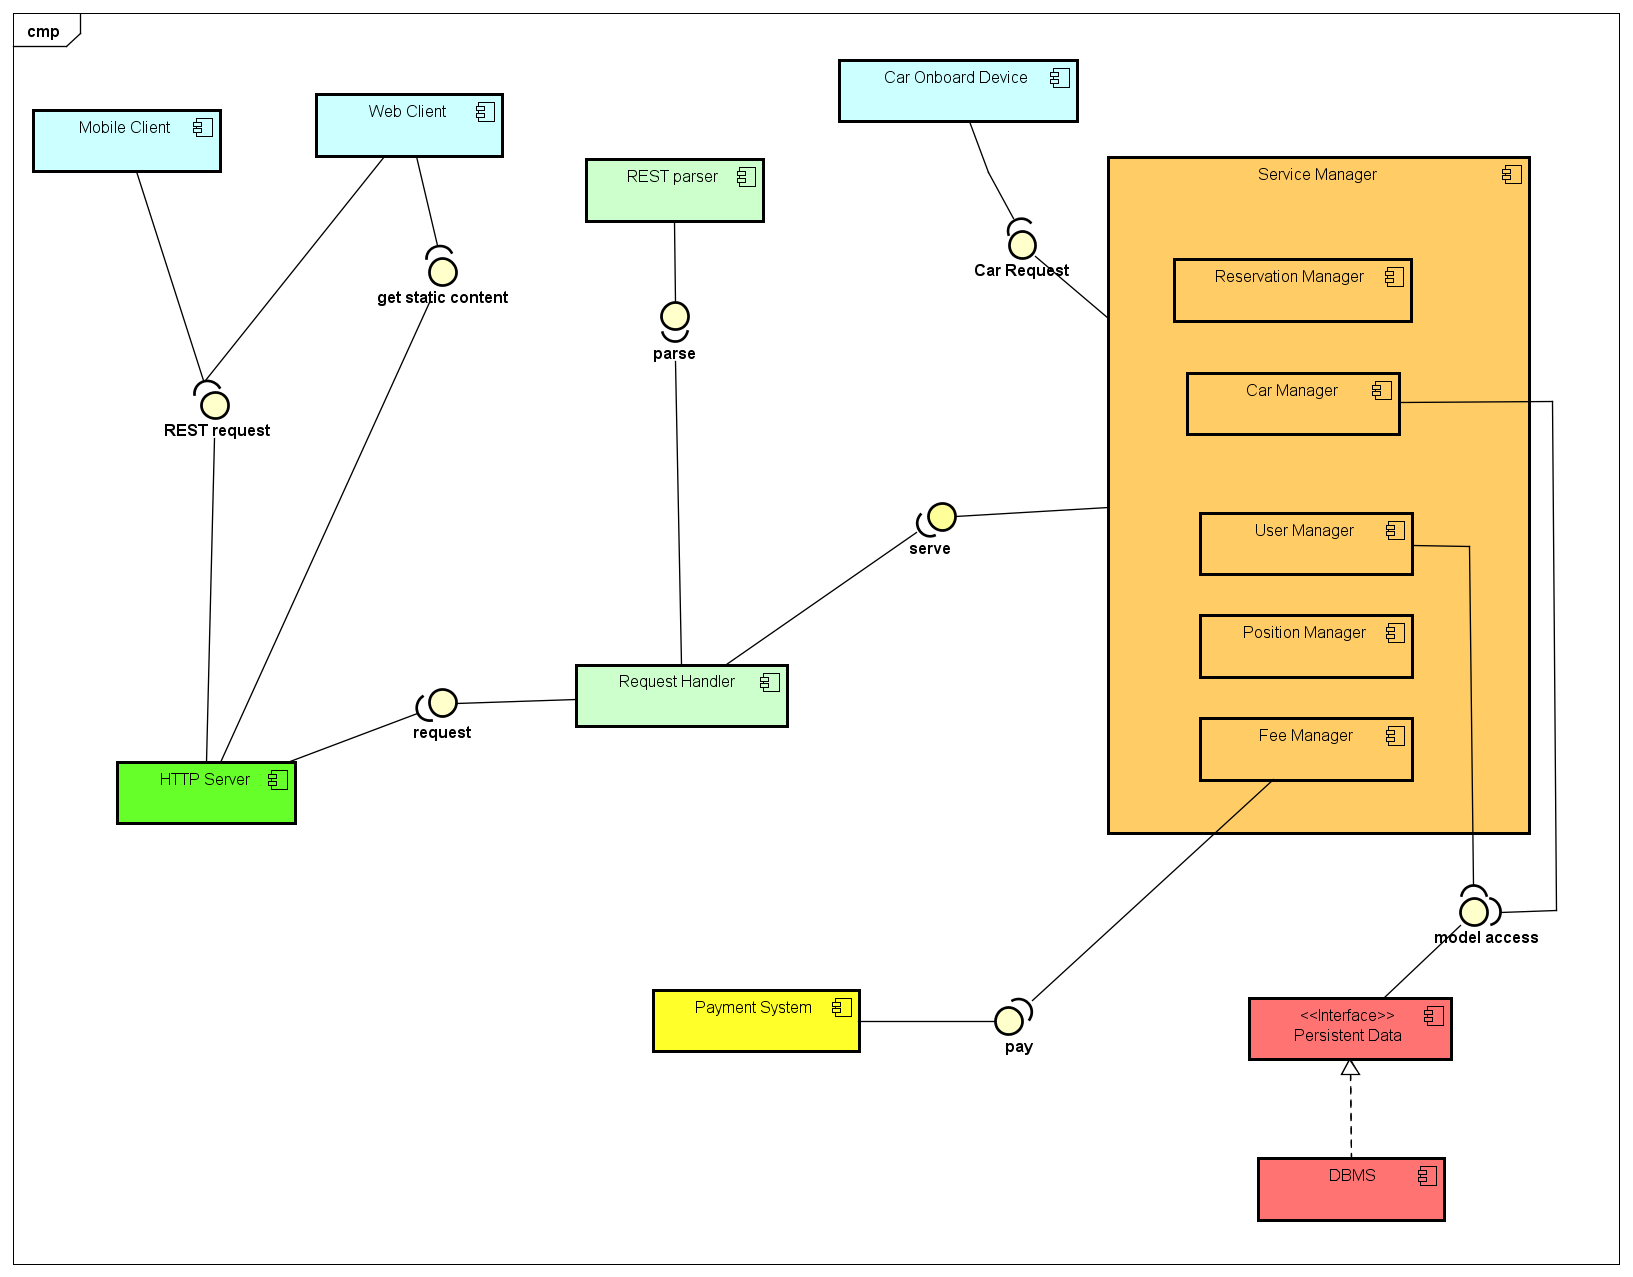
\includegraphics[width=\textwidth]{img/Component_Diagram}
	\caption{Component Diagram}
\end{figure}

The communication between the clients (both mobile application and web site) are realized using a request-response methodology. The client asks for information or to make actions related to the server using \textbf{REST} requests and obtains a response from the server formatted as a \textbf{JSON} object, today the state of the art for web services communications. 
All the REST requests received by the \textbf{HTTP Server} are forward to and, then, processed by the Request Handler component. The Request Handler component is in charge of validating the request integrity, parsing it using the \textbf{REST Parser} component and check the authentication for the requests type that need a valid session.

The OnBoard device of the car does not interact with the HTTP Server, but he has its own interface between it and the Service Manager, that forwards its requests to the Car Manager.

When a requests pass these checks is forwarded to the Service Manager where the application logic is applied.
The \textbf{Service Manager}, depending on the types of request that are received,  processes a response using Car Manager, User Manager, Position Manager, Trip Manager or Fee Manager.
Using those component the Service Manager can access the model, manage the request and craft a response.Every request can instantiate different component.

The system status are represented through various \textbf{Java Beans} object that stay alive for all the time needed for the request processing.

When a request is received all the element from the model needed for the processing are loaded from the persistent data storage through the \textbf{Persistent Data interface}. The abstraction exposed by the Persistent Data interface allow to adopt different data storage solution in a transparent way to the various component that are using it. All the persistent data are stored through a distributed database that can optimize data access.

\newpage

\subsection{Deployment view}\label{deployment}
 	
\begin{figure}[H]	
	\centering
	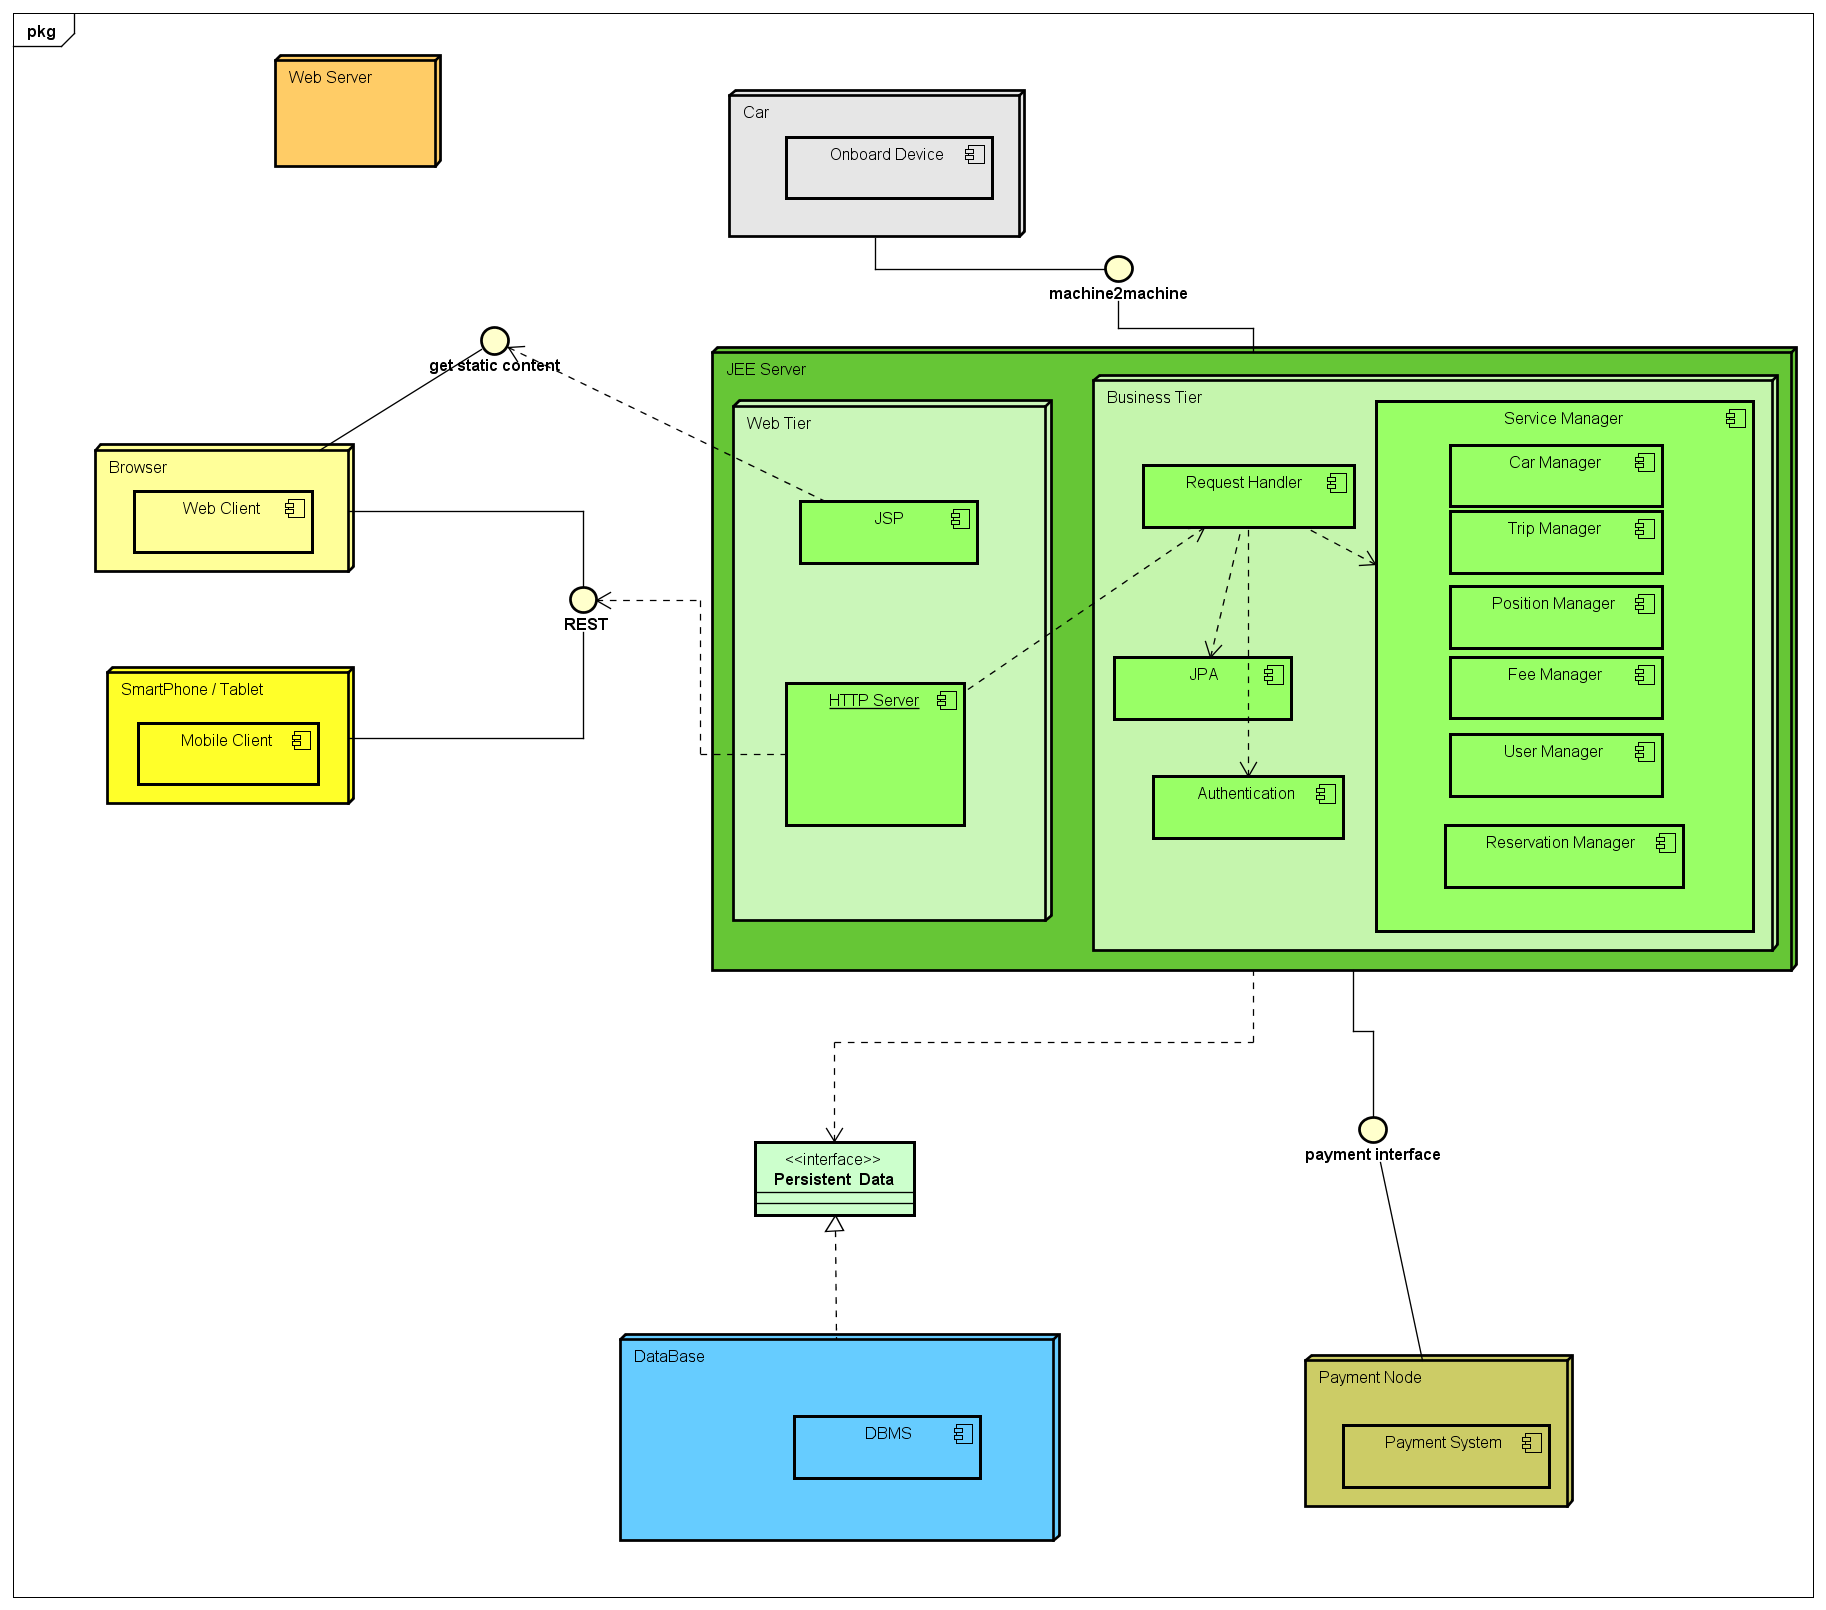
\includegraphics[width=\textwidth]{img/deployment_diagram}
	\caption{Deployment Diagram}
\end{figure}

From the deployment perspective, the components described in the Component view will be installed on 3 different machines:

\begin{itemize}
\item \textbf{JEE Server}: On this machine will be installed a Glassfish server, that is an oper source application server supporting JEE. This Server will contain all the components handling the business and the web logic.
\item \textbf{Database}: On this machine will be stored all the persistent data. On the database will be installed the latest version (5.6) of MySQL, a relational DBMS distributed by Oracle, that will handle the creation, deleting and updating of the tables of the databases containing the data.
\item \textbf{Client}: This machine is the one that the user will use to use the Power EnJoy service. It can be a Mobile Device, so a SmartPhone or a Tablet, a PC or the OnBoard Device. On the Mobile Device will run the Mobile Application. If the user uses a PC instead, he will access the service using the WebSite, that runs on any kind of Browser. Lastly, when the user is driving, the Client machine will be the OnBoard Device, that is the device mounted on the Car, on which will run a proprietary software of Power EnJoy.
\end{itemize}

\newpage

\subsection{Runtime view}
In this section we show the runtime behaviour of the system in various situations, in order to show which components have to act and how they interact.
\begin{figure}[H]	
	\centering
	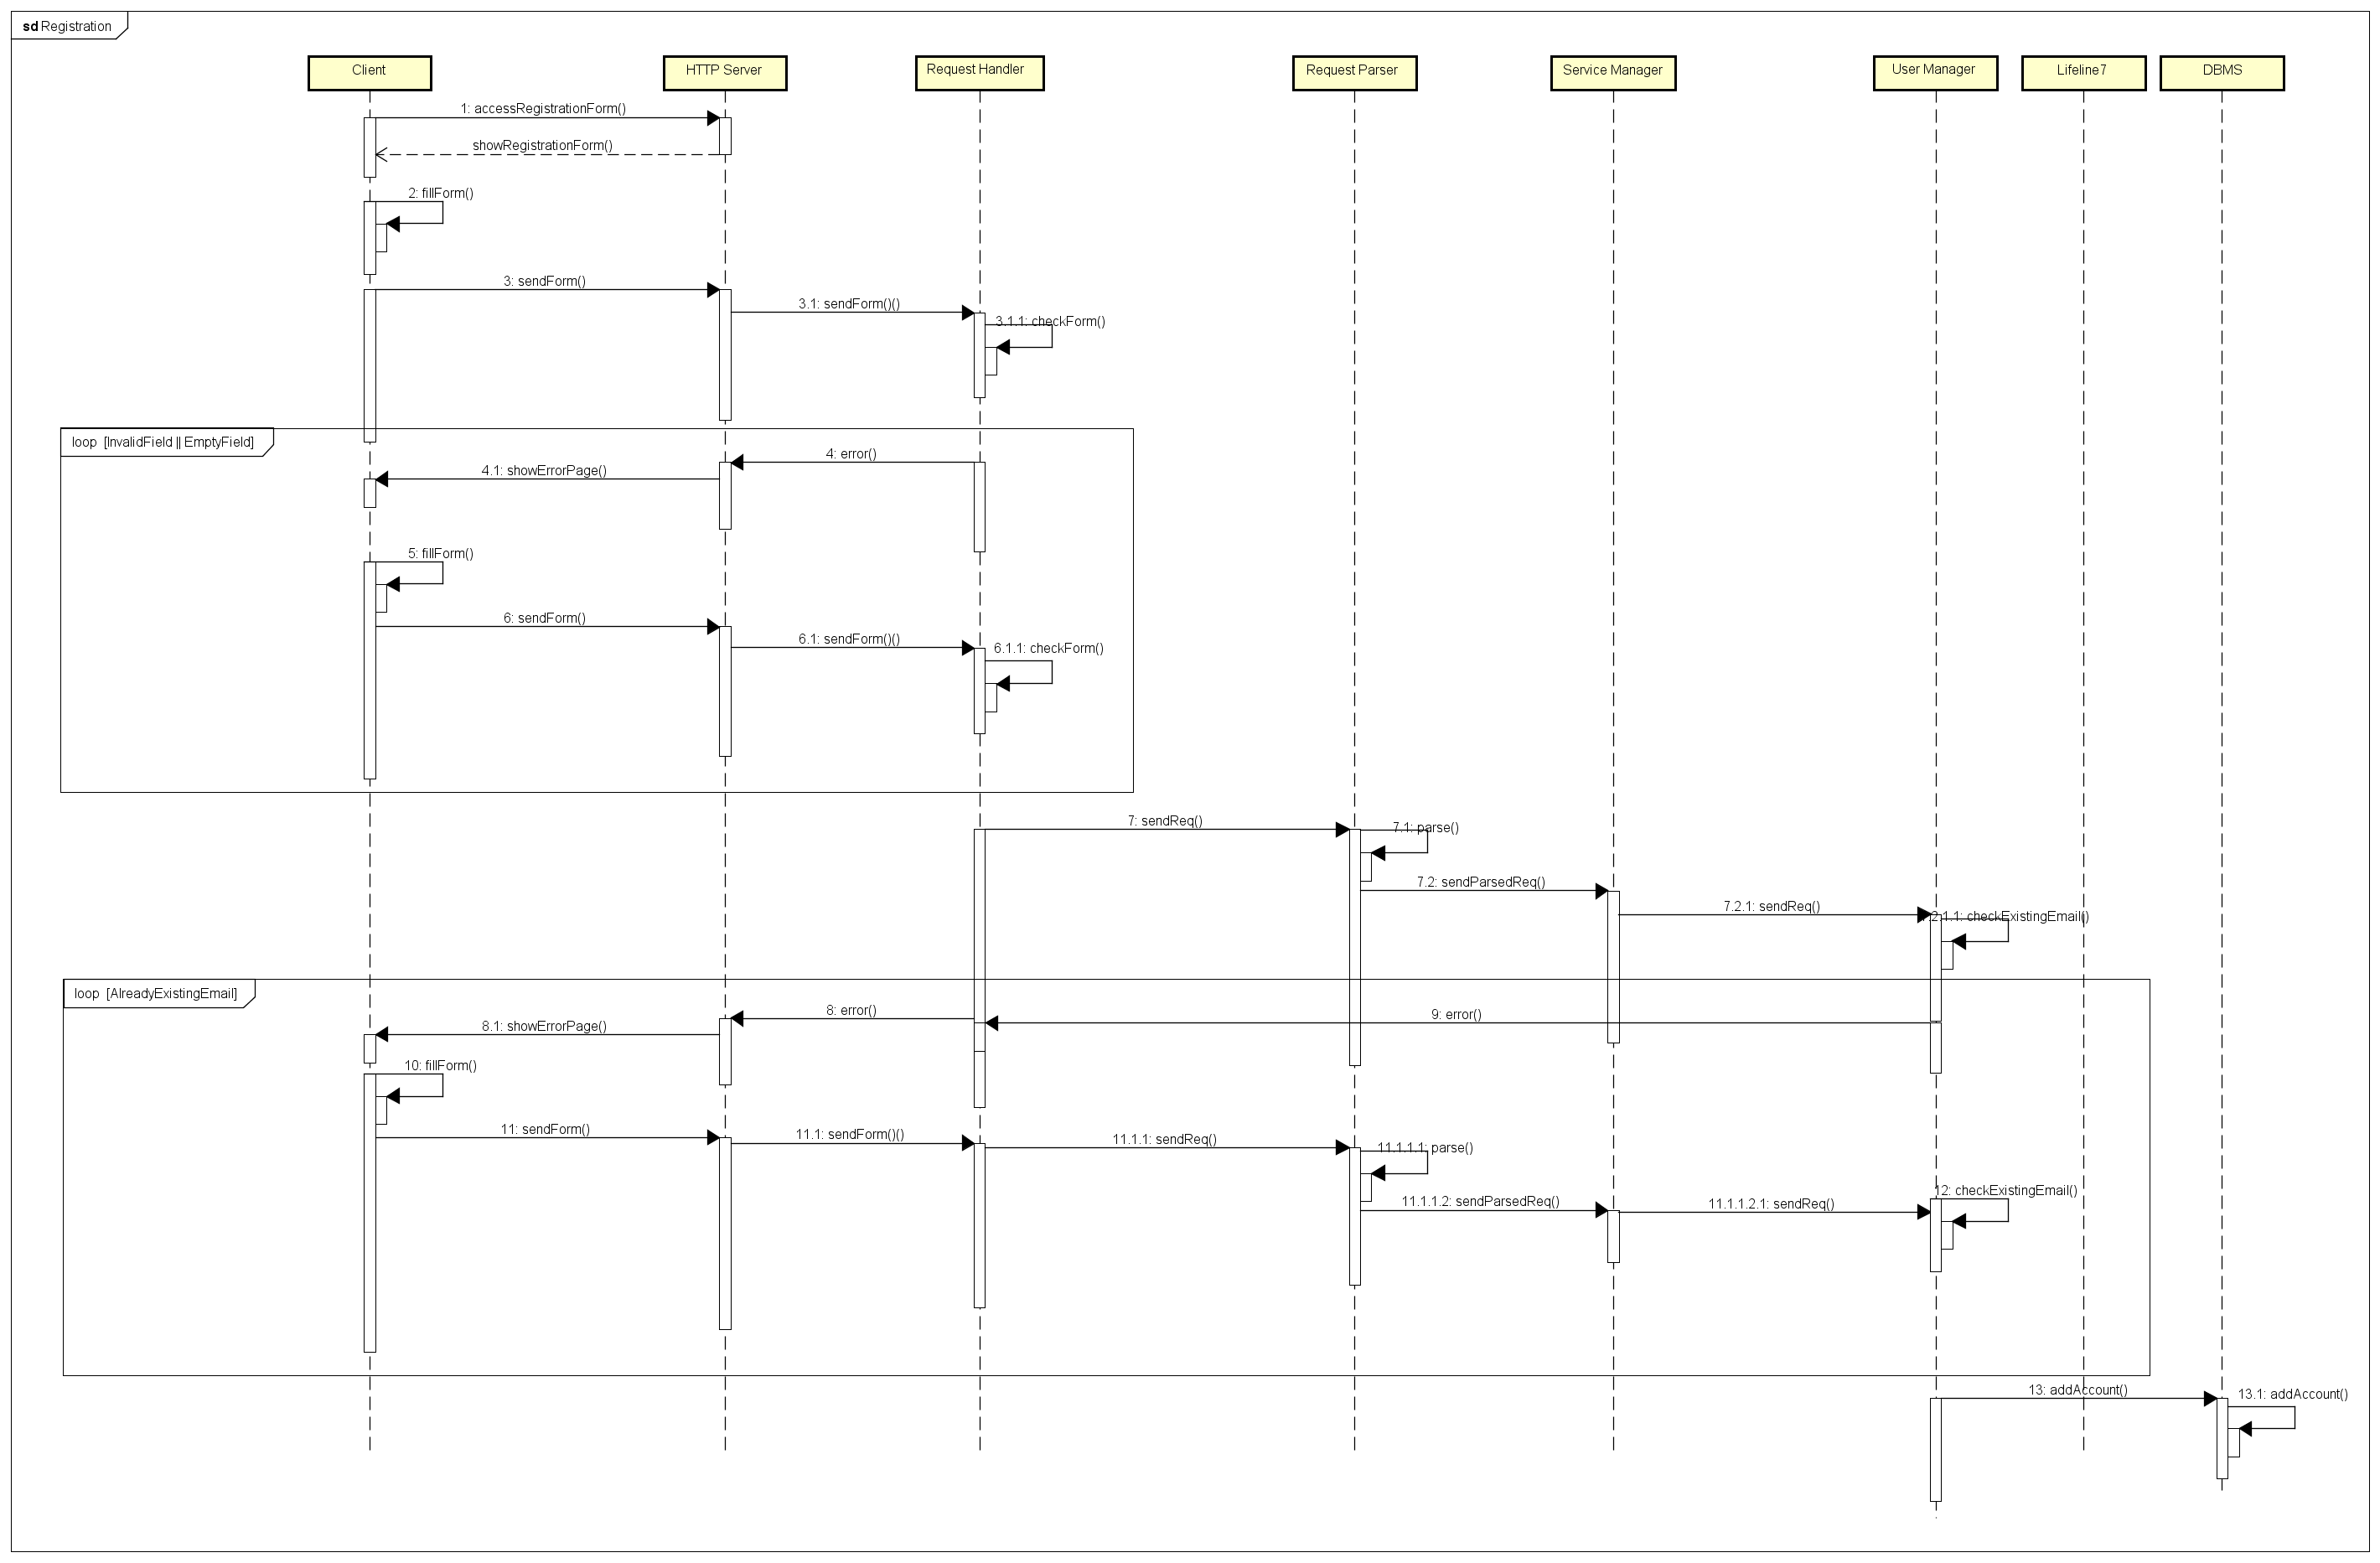
\includegraphics[width=\textwidth]{img/sequence_registration}
	\caption{Sequence Diagram of the Registration process}
\end{figure}
\newpage

\begin{figure}[H]	
	\centering
	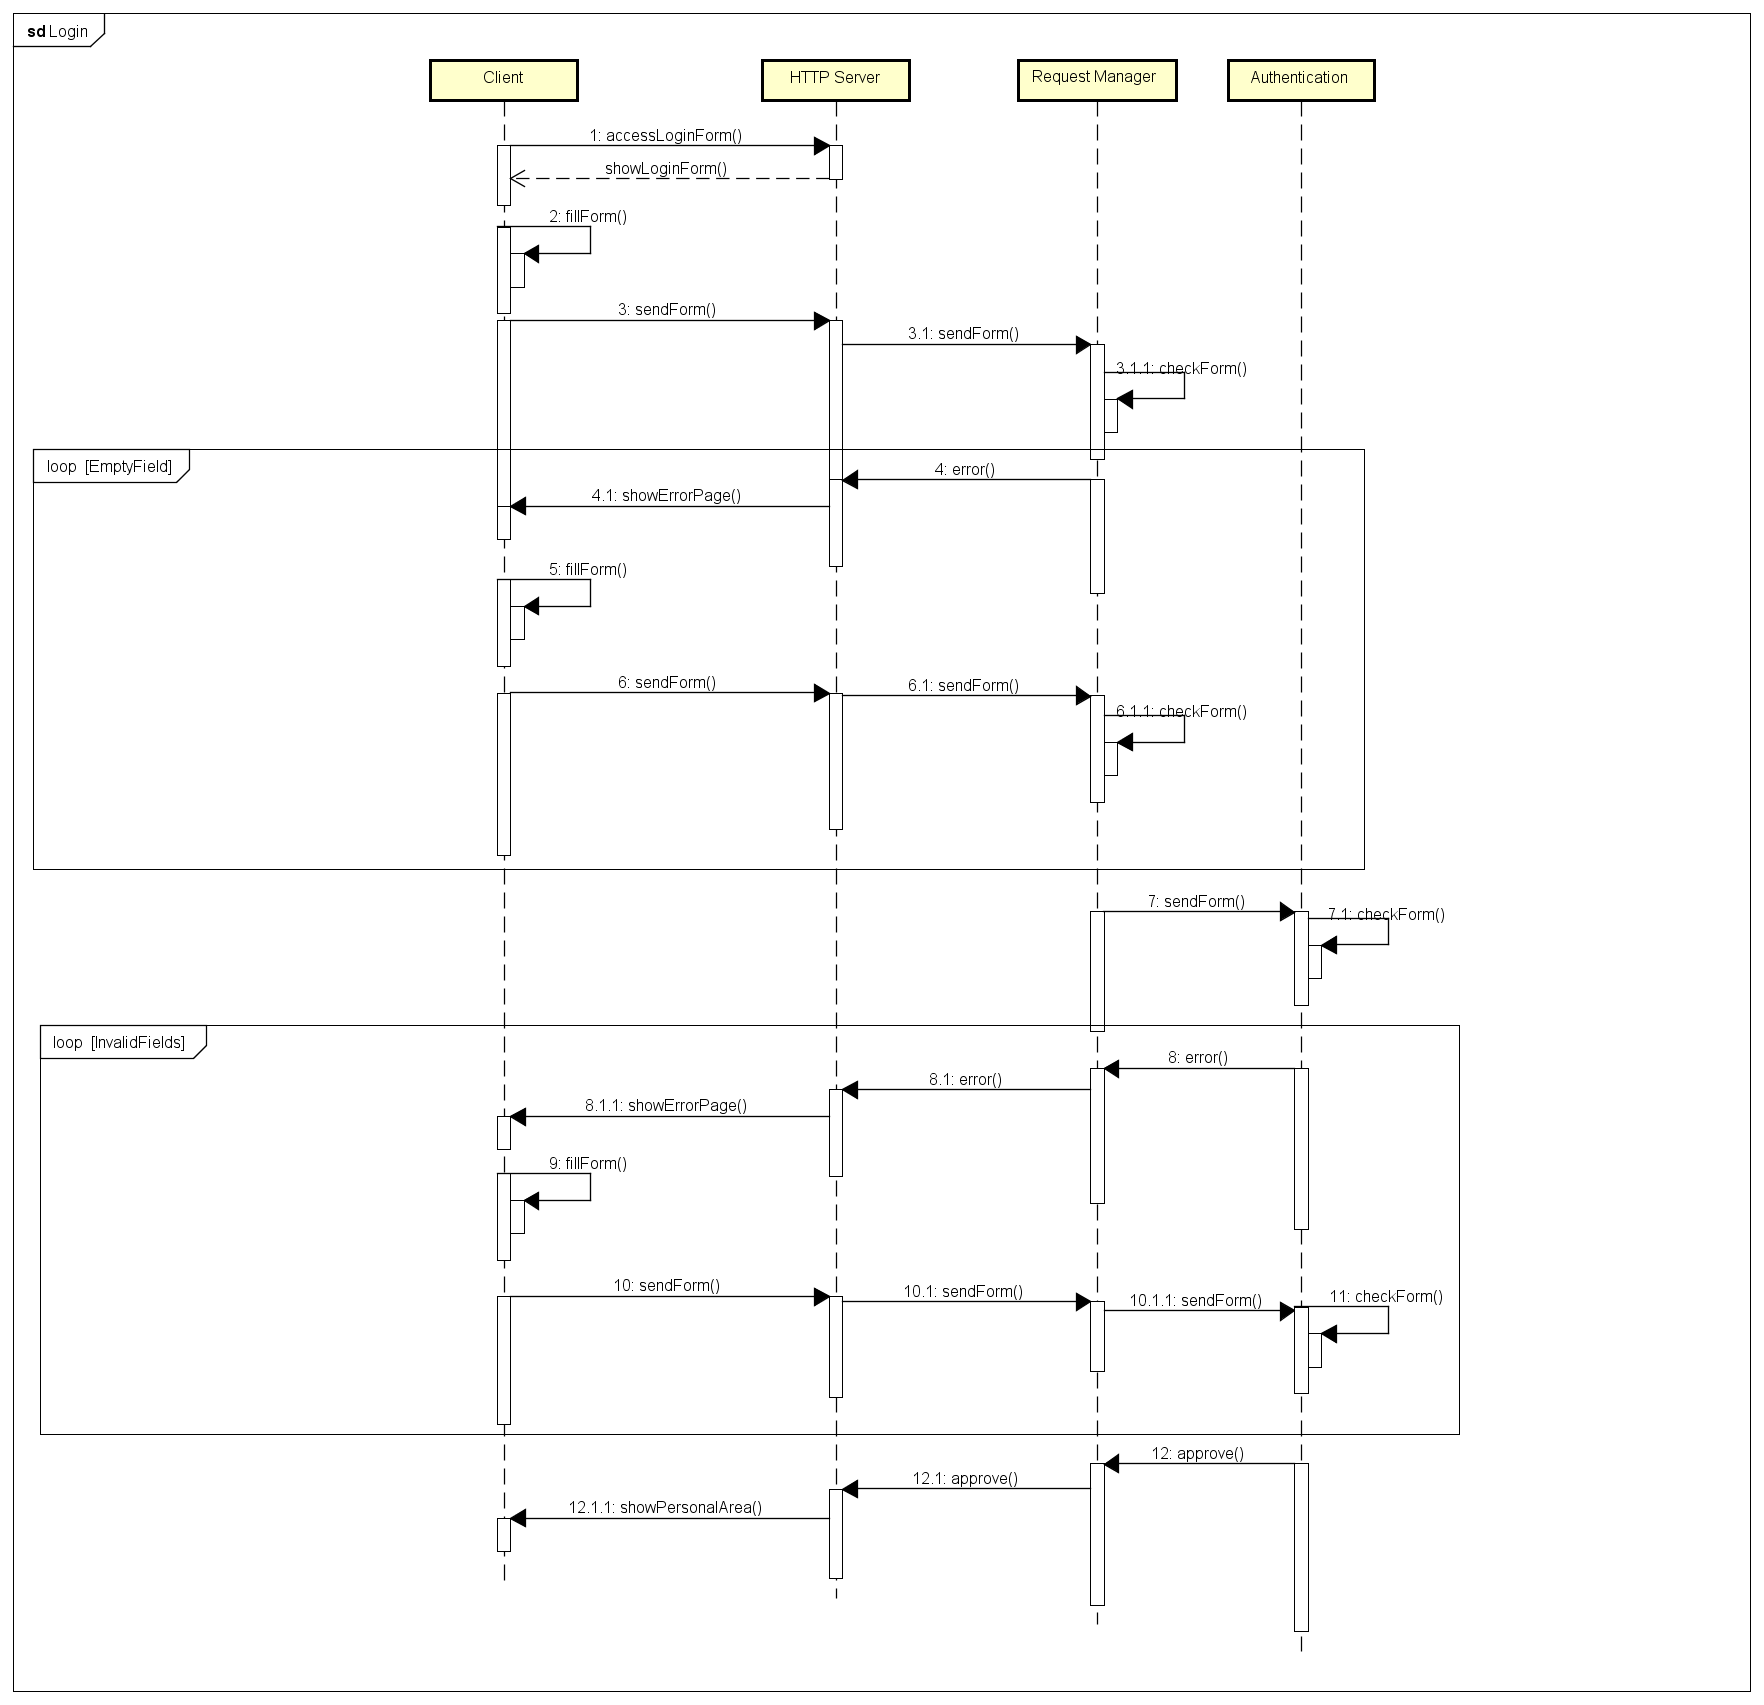
\includegraphics[width=\textwidth]{img/sequence_login}
	\caption{Sequence Diagram of the Login process}
\end{figure}
\newpage

\begin{figure}[H]	
	\centering
	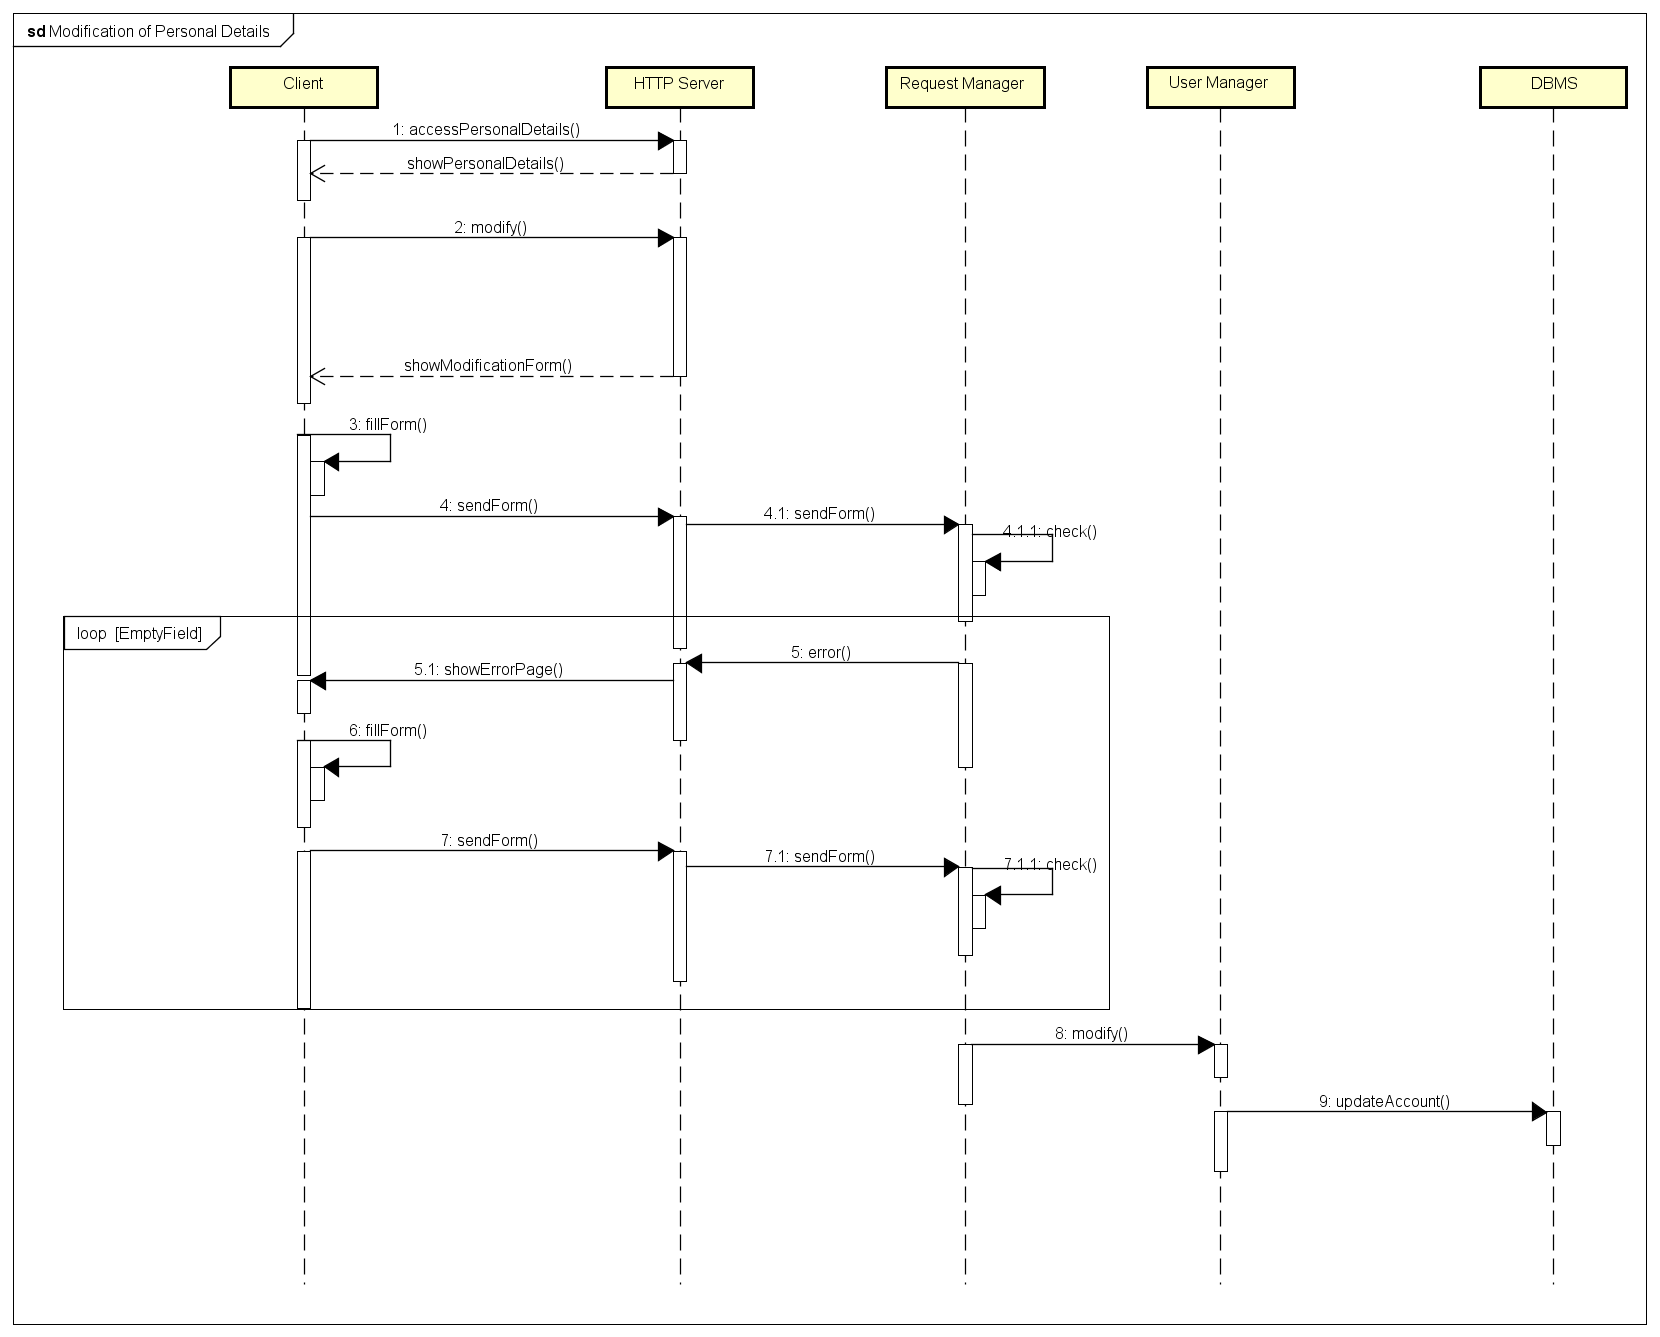
\includegraphics[width=\textwidth]{img/sequence_modification}
	\caption{Sequence Diagram of the Modification of Personal Details process}
\end{figure}
\newpage

\begin{figure}[H]	
	\centering
	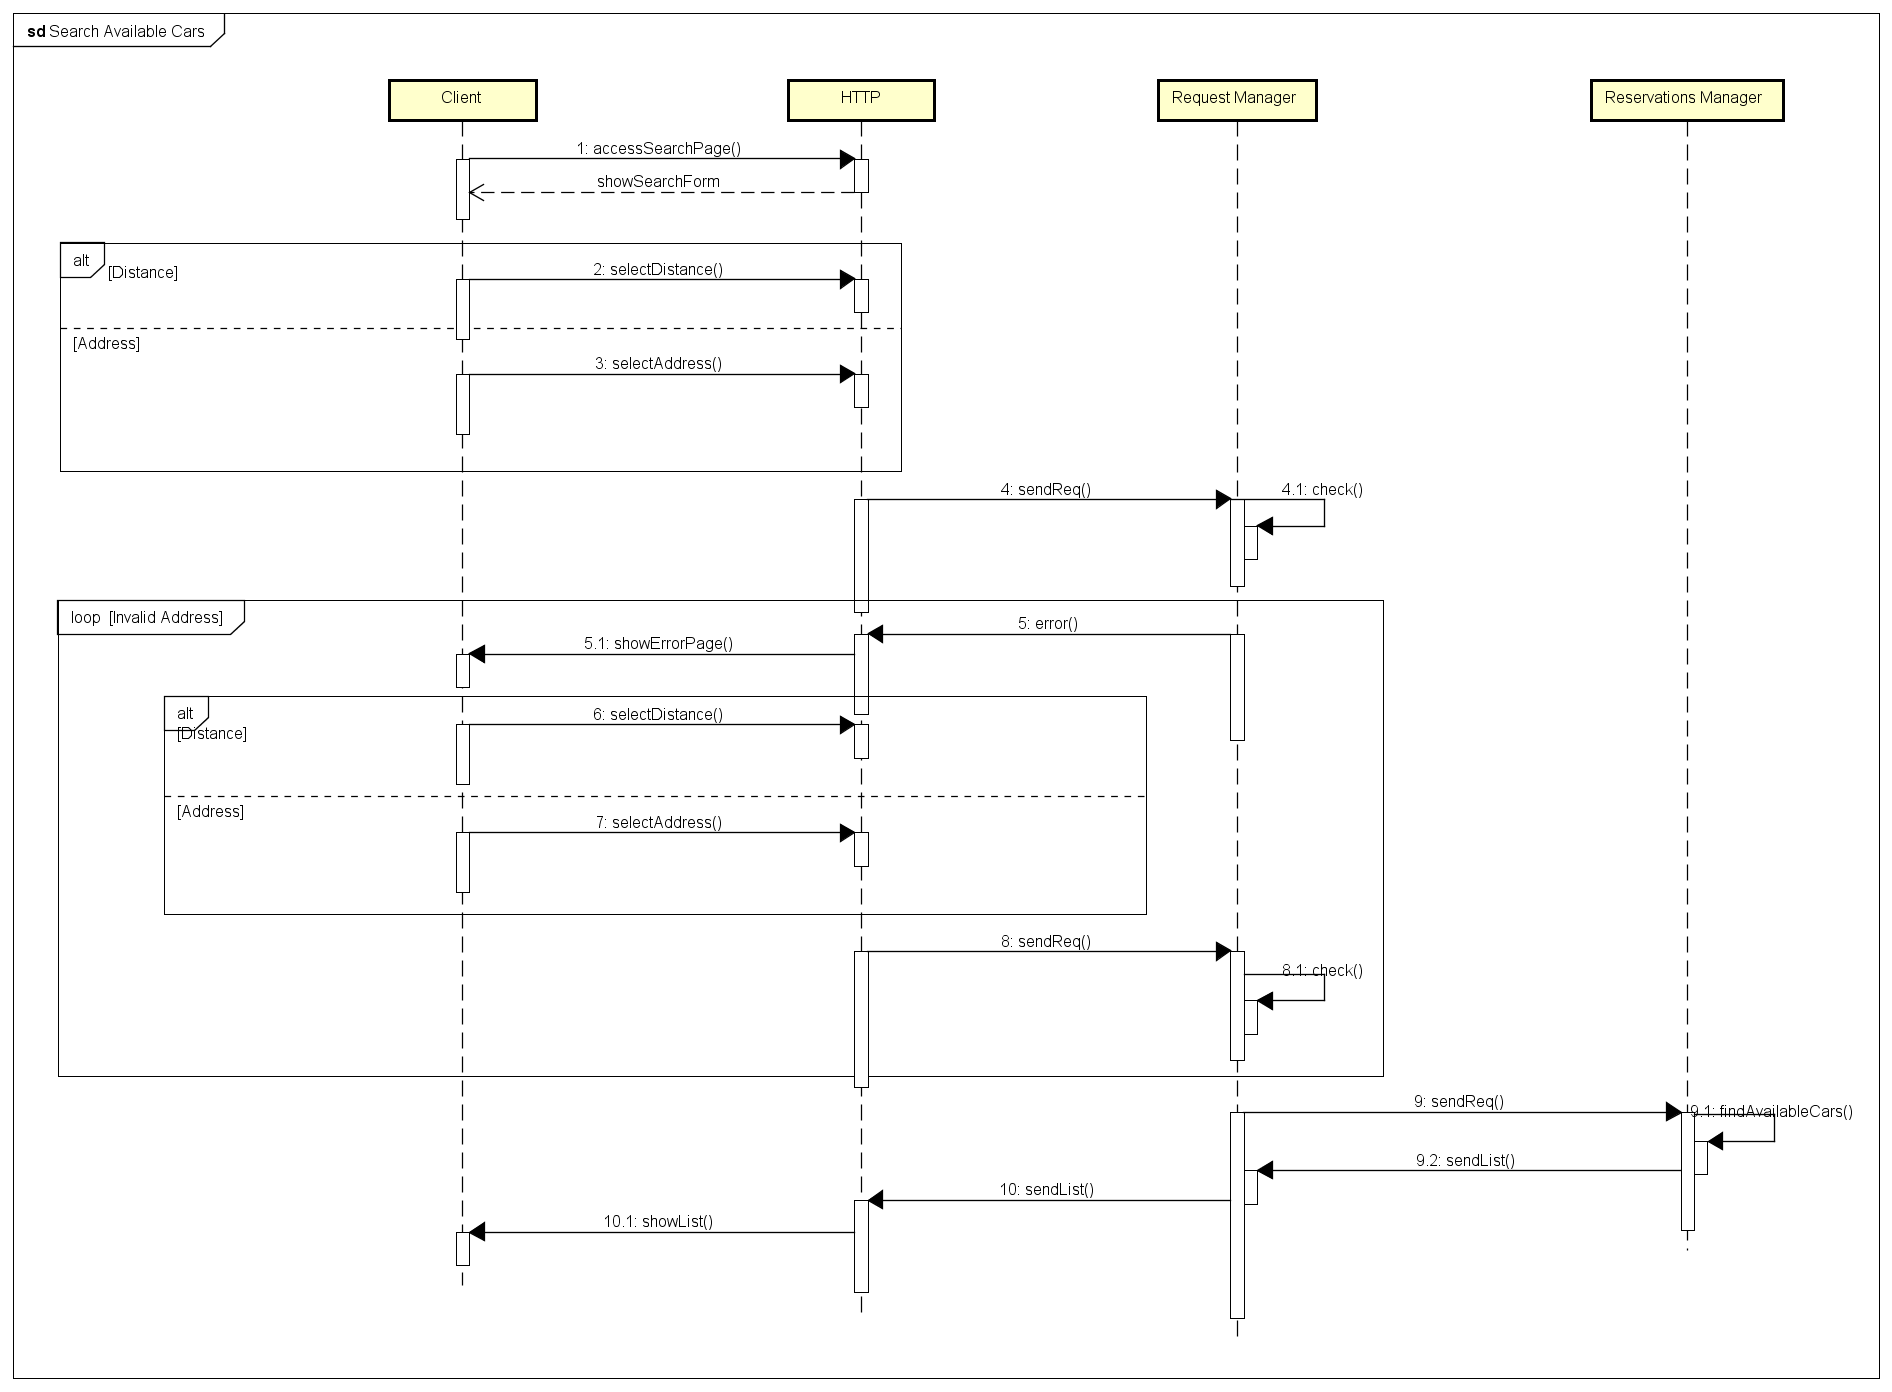
\includegraphics[width=\textwidth]{img/sequence_search}
	\caption{Sequence Diagram of the Search of Available Cars process}
\end{figure}
\newpage


\begin{figure}[H]	
	\centering
	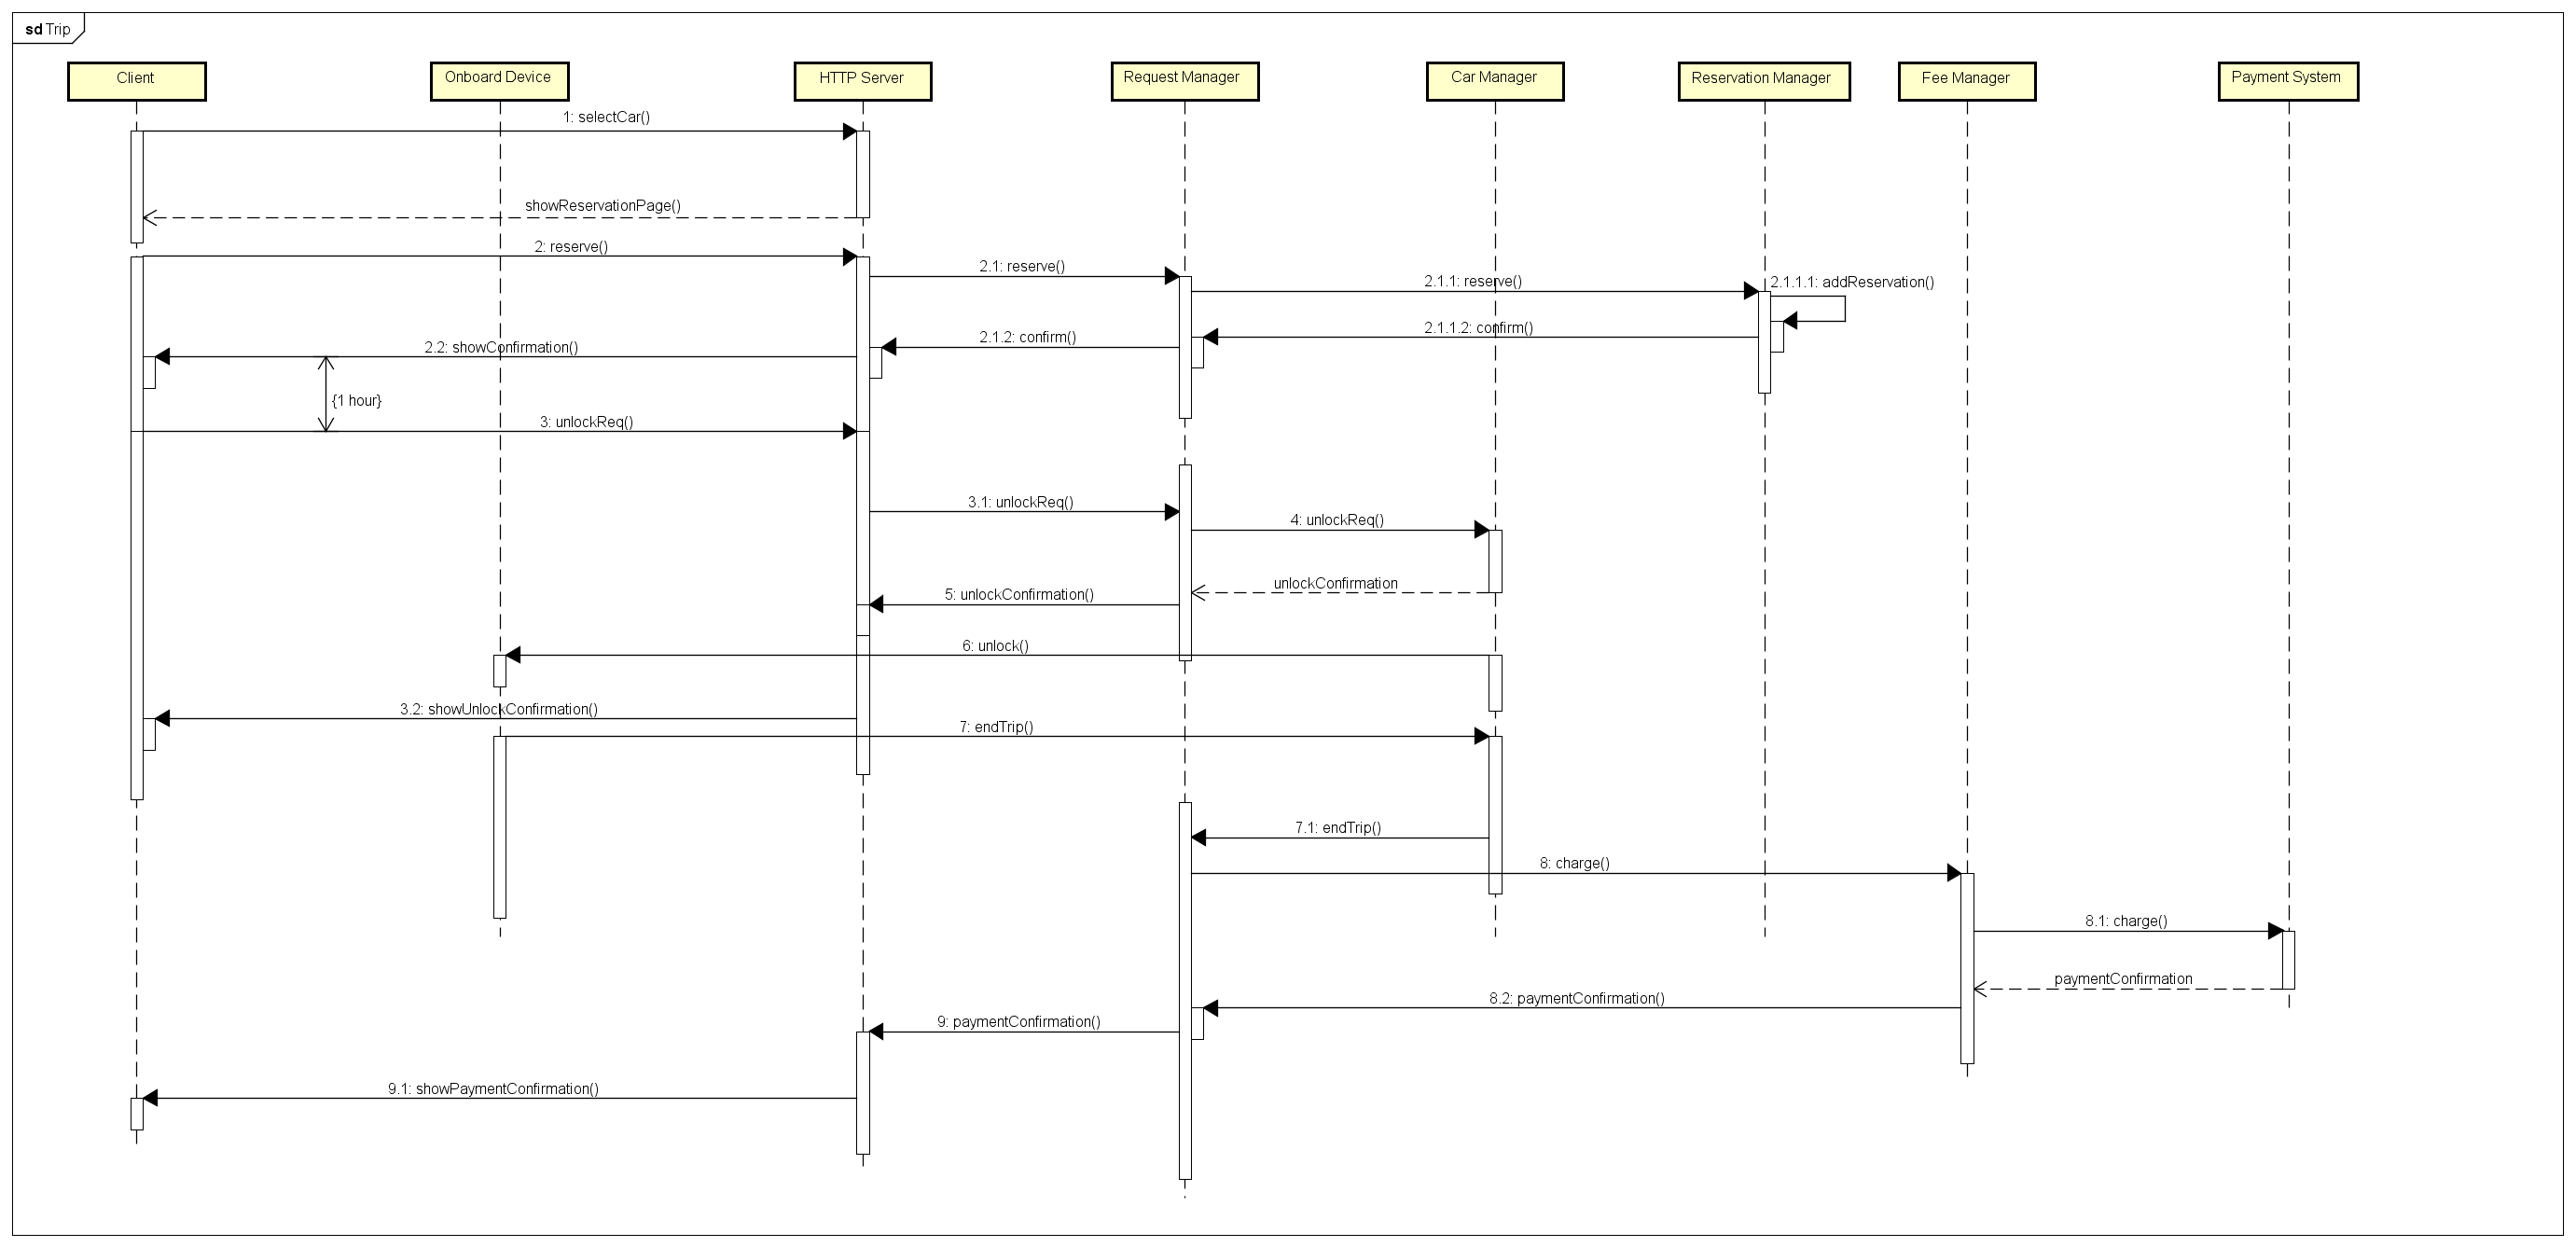
\includegraphics[width=\textwidth]{img/sequence_trip}
	\caption{Sequence Diagram of the Trip process}
\end{figure}
\newpage



\subsection{Component interfaces} 
\subsubsection{REST}
As explained in the introduction the communication takes place via REST requests. The REST model establish a relation map between the common CRUD operations (Create, Read, Update and Delete of a resource) and the HTTP operations as explained in the following table.

\begin{center}
	\begin{adjustbox}{max width=\textwidth}	
		\begin{tabular}{|l|>{\raggedright}p{2.5cm}|>{\raggedright}p{4.5cm}|>{\raggedright}p{5cm}|}
			\hline 
			CRUD & REST Http & example &description\tabularnewline
			\hline 
			Create & POST/PUT & POST /user/register  & Create a resource \tabularnewline
			\hline 
			Read & GET & GET /cars/zone/12 & Retrieve information. \\  Requests must be safe and idempotent.\tabularnewline
			\hline 
			Update & PUT & PUT /user/gpsposition & Update an existing entity. Request is idempotent. \tabularnewline
			\hline 
			Delete & DELETE & DELETE /car/request/28 & Remove a resource.\tabularnewline
			\hline 
		\end{tabular}
	\end{adjustbox}	
	\captionof{table}{Rest/CRUD interface mapping.}
	\par\end{center}

\subsubsection{Database Connectivity} \textbf{JDBC} (Java Database Connectivity) is used as connector between Database and the Application Server. JDBC, in fact, is a software component that allows Java applications to interact with databases. It has been chosen because have support for almost every \textbf{DBMS} on the market.
To enhance the connection, JDBC requires drivers for each database. These drivers connect to the database and implement the protocol to query and get respective results between the client and database. 


\textbf{ODBC} driver is a level of abstraction that allows programmers to make SQL requests to access data from distinct Database without having to know the proprietary interfaces of each DB. In this way it is easier to change the database without altering the application layer.


\begin{figure}[H]	
	\centering
	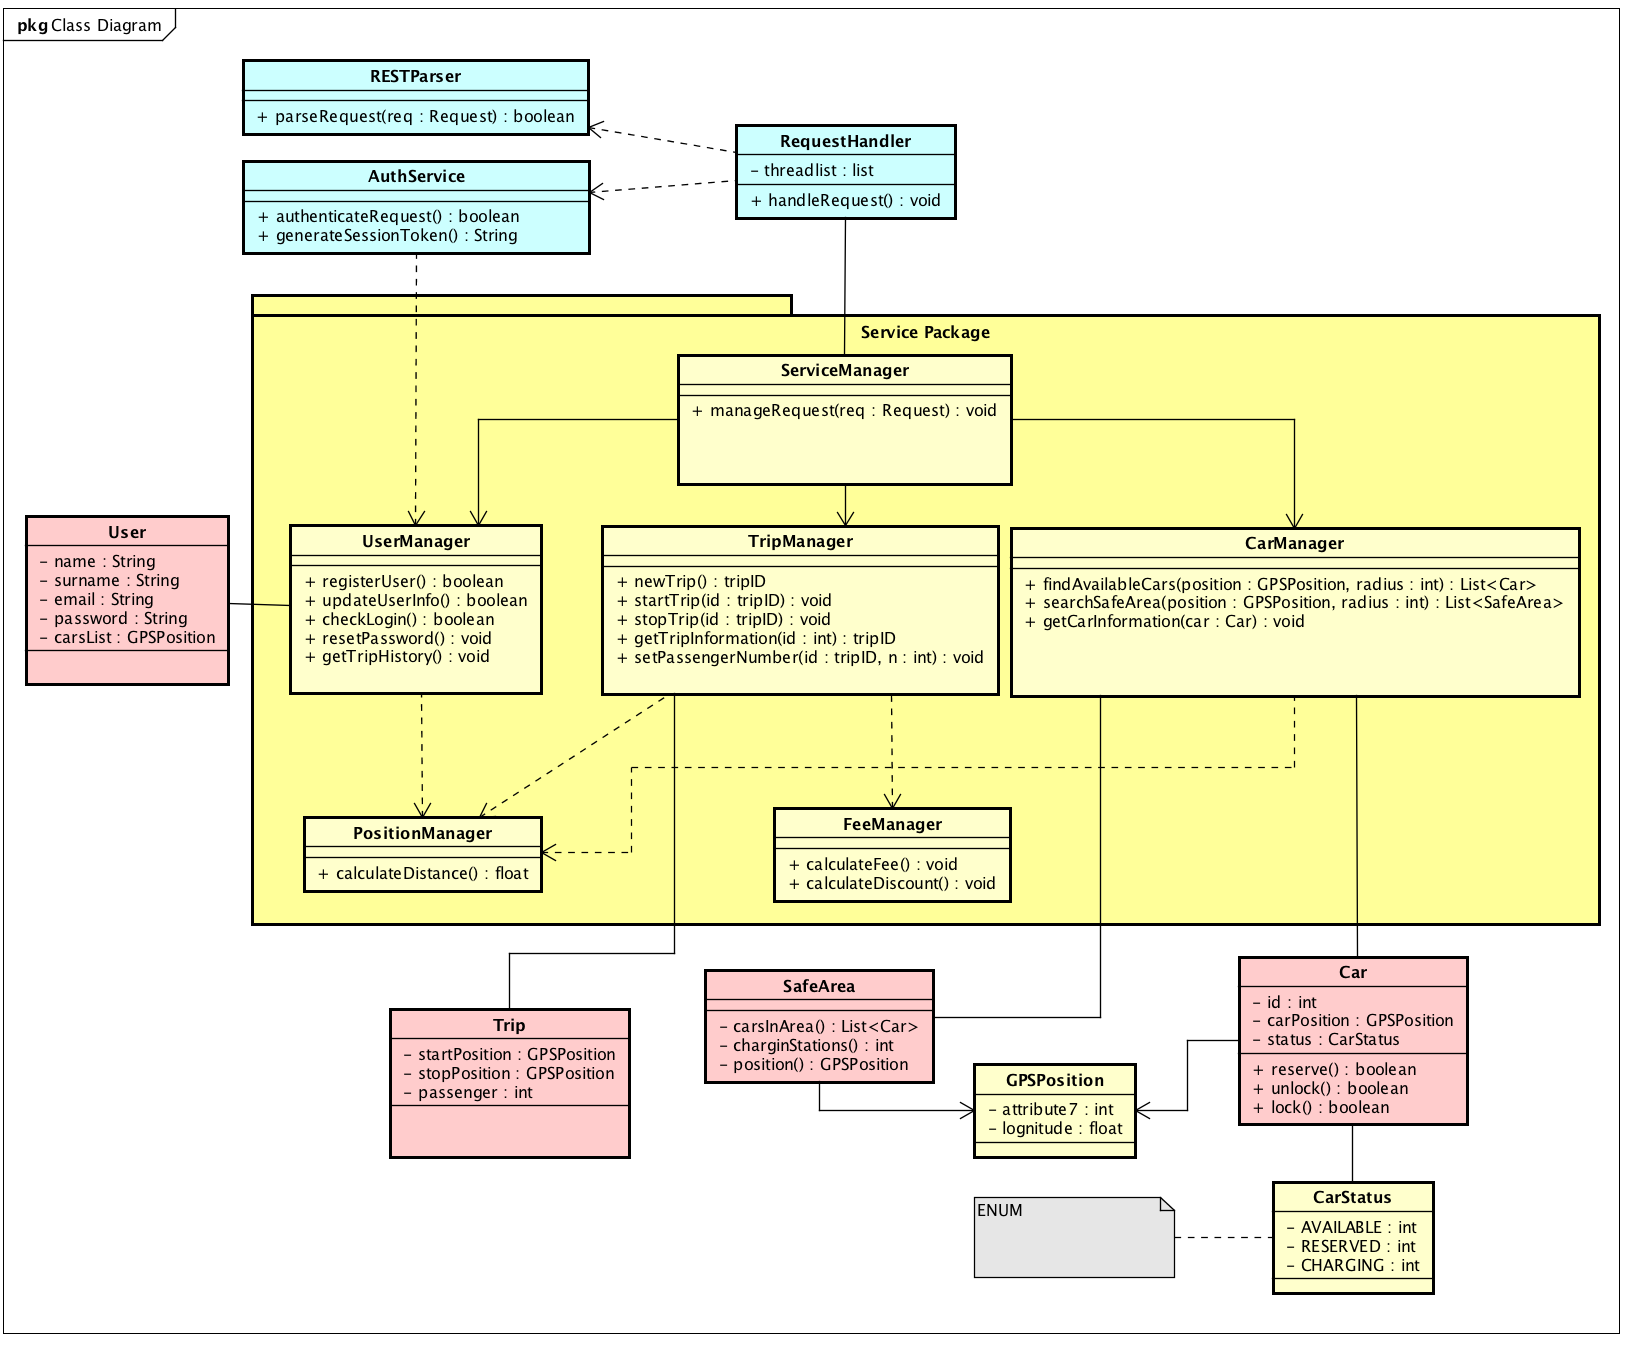
\includegraphics[width=\textwidth]{img/class_diagram}
	\caption{Class Diagram}
\end{figure}

\subsubsection{Backend Component Interface Description}
\begin{itemize}
	\item{\textbf{ServiceManager:}
		The Service Manager is instantiated when a new request has been parsed and validate.
			\begin{itemize}
				\item \textit{manageRequest(Request)}: Receive as input a new request and instantiate the right component to manage it.
			\end{itemize}
		}
	\item{\textbf{UserManager:}
	The User Manager is instantiate when ad User action or an User information are required.
	\begin{itemize}
		\item \textit{registerUser()}: Check if provided informations are correct and create a new User entity in the model.		
		\item \textit{updateUserInfo()}: Update the selected User entity in the model.
		\item \textit{checkLogin()}: Check if provided informations are correct and allow to create a new Session.
		\item \textit{resetPassword()}: Send to the User email a link to reset the account password.
		\item \textit{getTripHistory()}: Get a list of the User's past trip.
	\end{itemize}
}
	\item{\textbf{TripManager:}
	The Trip Manager is instantiate when the User start or end a trip.
	\begin{itemize}
		\item \textit{newTrip()}: Create a new Trip instance in the Model. Return a tripID.
		\item \textit{startTrip(tripID)}: Set the Trip starting position.
		\item \textit{stopTrip(tripID)}: Set the Trip ending position.
		\item \textit{getTripInformation(tripID)}: Return the information about a specific Trip (past or current).
		\item \textit{setPassengerNumber(tripID, int n)}: Set the passengers number for a specific Trip.
	\end{itemize}
}
	\item{\textbf{CarManager:}
	The Car Manager is instantiate when to manage cars request or get a specific car status.
	\begin{itemize}
		\item \textit{findAvailableCars(GPSPosition,radius)}: Return a set of cars in a given radius centered on a GPS position.
		\item \textit{searchSafeArea(GPSPosition,radius)}: Return a set of SafeArea given radius centered on a GPS position.
		\item \textit{getCarInformation(Car)}: Return the status of a specific car (example the charge of the battery).
	\end{itemize}
}
	\item{\textbf{PositionManager:}
	The Position Manager is used when a calculation between GPS Coordinate is needed.
	\begin{itemize}
		\item \textit{calculateDistance(GPSPosition,GPSPosition)}: Return a cartesian distance between two coordinate.
	\end{itemize}
}
	\item{\textbf{FeeManager:}
	The Fee Manager is instantiate to calculate the amount of money that need to charge to the user.
	\begin{itemize}
		\item \textit{calculateFee(tripID)}: Calculate the normal fee for the trip in base of the time and distance traveled.
		\item \textit{calculateDiscount(tripID)}: Apply a discount in base of starting/ending position and state of the car after the travel and the number of passenger.
	\end{itemize}
}

	\item{\textbf{RequestHandler:}
	The Request Handler select a free thread from an allocated pool to handle an HTTP request.
	\begin{itemize}
		\item \textit{handleRequest()}: Use the REST parser and the AuthService to validate a request.
	\end{itemize}
}

	\item{\textbf{AuthService:}
	The Authentication Service check if an User session for the request is valid.
	\begin{itemize}
		\item \textit{authenticateRequest()}: Check if a valid session token is provided for the request.
		\item \textit{generateSessionToken()}: Generate a session token to allow user to authenticate the requests.
	\end{itemize}
}
	\item{\textbf{RESTParser:}
	The REST Parser check te format of the REST request and discard a request if invalid
	\begin{itemize}
		\item \textit{parseRequest()}: Check if the request is valid.
	\end{itemize}
}
\end{itemize}

\newpage

\subsection{Selected architectural styles and patterns}

\subsubsection{Architecture}

We realized a 3-tiered architecture. In particular there are 3 dedicated machines for:

\begin{itemize}
\item Data Layer
\item Presentation Layer
\item Web Server and Application Server
\end{itemize}

The reader can see the organization of Tiers in details in \ref{deployment} \newline

 The reasons why we made this choice concern:

\begin{itemize}
\item {\textbf{Security:}} Is possible to setup a DMZ for the webserver and filter malicious requests before they reach the application server.
\item {\textbf{Scalability:}} Because of the separation of the layers, developers can modify existing functions or introduce new ones in any level (presentation, logic or data), leaving the other layers untouched.
\item {\textbf{Performance:} The webserver do a massive use of cache and load balancer to serve only static content to minimize resource and traffic}
\item {\textbf{Reliability and Available:}} because of the partition of tasks in distinct machines, it's easier to check for failures and fix them. So the time the system is down for maintainance is reduced and, as conseguence, the time the system is operating properly and the probability to find a system ready to accomplish users requests is increased. Furthermore, reliability and availability can be further improved further by replicating the servers, so that a failure in a single server doesn't affect the operativity of the system,  but only temporary reduces performances.
\end{itemize}


\subsubsection{Patterns}

\begin{itemize}
\item {\textbf{Client-Server:}} According to this pattern, in the system there should be 2 entities: a Client, that sends requests, and a Server, that elaborates requests and sends back results to the client. In our architecture there 3 Clients: the Mobile Client, the Web Client and the Driver Client. These all three  clients send requests to the \st{Web Server}HTTP server on the Application server, that takes care of forward it to the Request Handler and send back and show to the clients the results.


\item{\textbf{Model-View-Controller:}} In the MVC pattern there are 3 entities: The Model, that contains methods to access the data, the View, that shows data to the user and allow him to perform actions, and the Controller, that elaborates the commands sended by the view manipulating and modifying  the data of the model.
In our system the View is the Client, the Model is the Data Manager and the Controller is the Service Manager. Furthermore, between the View and the Controller we have put 2 middle components, to improve the quality and the performance of the system. The Web Server act as a request receiver and sends the commands of the View to the Request Handler. The Request Handler act as validator and activates the forwarding of the command to the Controller only if the request respects integrity and authentication constraints.

\item{\textbf{Resource Injection:}} Because of the amount of users , it is useful to have a mechanism that can inject objects in an application at runtime, so that the application hasn't to care about the creation of object everytime he needs it. So we decided to use JNDI service to name and lookup for resources and the Resource Injection mechanism provide by JEE, that allows to inject any resource in the JNDI into an object.


\end{itemize}


